The goal for the Supermario model is to solve a level successfully. The first level was chosen since it provides a diverse environment with different enemy types and obstacles, while not being too skill intensive to solve. 
Prior to modeling some assumptions were made to fulfill time and complexity constraints.
Only a fixed number of enemies and obstacles in the path of the player are considered in order to ensure a static input size. For this number, five has proved to be sufficient for the first level and the implemented strategy. There are rarely more than 3 enemies in scene. For the same reason only the next hole in the ground is considered.
In order to develop the model, different situations were assessed and according tests derived. Both the scenarios which a Supermario model has to master and the derived tests are listed below.

\begin{figure}[!h]
	\centering
	
\includegraphics[scale=0.55]{pictures/haller_mario1.PNG}
	\caption{Mario has to jump and move right to overcome the obstacle}
	\label{fig:marioobstacle}
\end{figure}

Figure \ref{fig:marioobstacle} depicts the player next to an obstacle. In order to jump over it he has to move right and jump at the same time. He needs to keep jumping until he is higher than the obstacle.

\begin{figure} 
	\centering
    \subfigure[Mario evades a enemy by jumping]{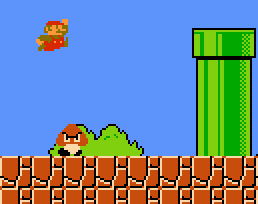
\includegraphics[height=0.3\textwidth]{pictures/haller_mario2.PNG}} 
    \subfigure[Mario defeats enemies by landing on them]{
\includegraphics[height=0.3\textwidth]{pictures/haller_mario3.PNG}} 
	\caption{Mario has to jump over/to enemies} 
	\label{fig:marioenemies}
\end{figure} 

Figure \ref{fig:marioenemies} shows two situations. In the first one, mario jumps to evade an enemy. The second depicts him landing on top of enemies to kill them.

\begin{figure} 
	\centering
    \subfigure[Mario and a hole in the ground]{
\includegraphics[height=0.3\textwidth]{pictures/haller_mario4.PNG}} 
    \subfigure[Mario and a hole with obstacles]{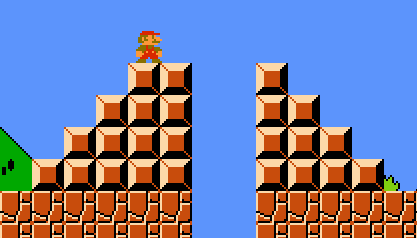
\includegraphics[height=0.3\textwidth]{pictures/haller_mario5.PNG}} 
	\caption{Mario has to jump over a hole} 
	\label{fig:mariohole}
\end{figure} 
In Figure \ref{fig:mariohole} the player is seen standing next to holes in the ground. In the first picture he is on the ground level, in the second he is standing on an obstacle.

The stream tests derived from the scenarios are introduced in the following.
\begin{lstlisting}[label=lst:enemywatchertest_1, caption=Enemy watcher stream test, morekeywords={package, stream, tick, for},
frame=single, basicstyle=\small, float,floatplacement=H]
package de.rwth.supermario.haller.environment;

stream Env_EnemyWatcher_Evade for EnemyWatcher {
    EnemyDistX:         200 tick    100     tick     75;
    EnemyDistY:           0 tick      0     tick      0;
    EnemyVelocityX:     -10 tick    -10     tick    -10;
    EnemyVelocityY:       0 tick      0     tick      0;
            
    movesTowardsPlayer:   1 tick      1     tick      1;
    inJumpRange:          0 tick      0     tick      1;
    }
\end{lstlisting}
If a enemy gets closer than 80 pixels (two blocks) and is on the same height as the player, the player has to jump in order to evade the enemy (listing \ref{lst:enemywatchertest_1}). The units for the EnemyDistX and EnemyDistY values are pixels, while the velocities are given in pixels per time frame.
The output values are of type boolean.

\begin{lstlisting}[label=lst:enemywatchertest_2, caption=Enemy watcher stream test, morekeywords={package, stream, tick, for},
frame=single, basicstyle=\small, float,floatplacement=H]
package de.rwth.supermario.haller.environment;

stream Env_EnemyWatcher_FromAbove for EnemyWatcher {
        
    EnemyDistX:         200 tick    100     tick      5;
    EnemyDistY:         128 tick    128     tick     32;
    EnemyVelocityX:     -10 tick    -10     tick    -10;
    EnemyVelocityY:       0 tick      0     tick      0;
            
    movesTowardsPlayer:   1 tick      1     tick      1;
    inJumpRange:          0 tick      0     tick      0;

    }
\end{lstlisting}
The stream in listing \ref{lst:enemywatchertest_2} covers the case when the player is above enemies and shall drop on them while he is above.



\begin{lstlisting}[label=lst:enemywatchertest_3, caption=Enemy watcher stream test, morekeywords={package, stream, tick, for},
frame=single, basicstyle=\small, float,floatplacement=H]
package de.rwth.supermario.haller.environment;

stream Env_EnemyWatcher_FromAbove for EnemyWatcher {
        
    EnemyDistX:         -1 tick;
    EnemyDistY:         -1 tick;
    EnemyVelocityX:      0 tick;
    EnemyVelocityY:      0 tick;
            
    movesTowardsPlayer:  0 tick;
    inJumpRange:         0 tick;

    }
\end{lstlisting}
If there is no enemy near the player, the enemy watcher object shall give no jump advice (listing \ref{lst:enemywatchertest_3}).



\begin{lstlisting}[label=lst:obstaclewatchertest, caption=Obstacle watcher stream test, morekeywords={package, stream, tick, for},
frame=single, basicstyle=\small, float,floatplacement=H]
package de.rwth.supermario.haller.environment;
stream Env_ObstacleWatcher for ObstacleWatcher {
  ObstacleDistX: 200 tick 100 tick 75 tick 50 tick 25 tick  0;
  ObstacleDistX:   0 tick   0 tick  0 tick 25 tick 50 tick 75;
    
  inJumpRange:     0 tick   0 tick  1 tick  1 tick  1 tick  0;
    }
\end{lstlisting}
If a obstacle is in front of the player, he shall jump until he has passed it(listing \ref{lst:obstaclewatchertest}). The distances are given in pixels, and the obstacle in this text is of 70px height.

\begin{lstlisting}[label=lst:holewatchertest, caption=Hole watcher stream test, morekeywords={package, stream, tick, for},
frame=single, basicstyle=\small, float,floatplacement=H]
package de.rwth.supermario.haller.environment;
stream Env_ObstacleWatcher for ObstacleWatcher {
    holeDistance: 200 tick 100 tick 10 tick 0 tick 1200;
    
    inJumpRange:    0 tick   0 tick  1 tick	1 tick    0;
    }
\end{lstlisting}

In listing \ref{lst:holewatchertest} the stream test for jumping over holes is given. In this case, the player shall start jumping close to the hole and only stop once he is over.


